\documentclass[
	12pt,
	a4paper,
	bibtotoc,
	cleardoubleempty, 
	idxtotoc,
	ngerman,
	openright
	final,
	listof=nochaptergap,
	]{scrbook}
\usepackage{cmap}
\usepackage[T1]{fontenc}
\usepackage[utf8]{inputenc}

% ##################################################
% Unterstuetzung fuer die deutsche Sprache
% ##################################################
%\usepackage{ngerman}
\usepackage[ngerman]{babel}
\usepackage{graphicx}
\usepackage{wrapfig}

% ##################################################
% Dokumentvariablen
% ##################################################

% Persoenliche Daten
\newcommand{\docNachname}{Mustermann}
\newcommand{\docVorname}{Max}
\newcommand{\docStrasse}{Straße}
\newcommand{\docOrt}{Ort}
\newcommand{\docPlz}{123456}
\newcommand{\docEmail}{student@hs-furtwangen.de}
\newcommand{\docMatrikelnummer}{000000}

% Dokumentdaten
\newcommand{\docTitle}{TITEL}
%\newcommand{\docUntertitle}{} % Kein Untertitel
\newcommand{\docUntertitle}{UNTERTITEL}
% Arten der Arbeit: Bachelorthesis, Masterthesis, Seminararbeit, Diplomarbeit
\newcommand{\docArtDerArbeit}{ART DER ARBEIT}
%Studiengaenge: Allgemeine Informatik Bachelor, Computer Networking Bachelor,
% Software-Produktmanagement Bachelor, Advanced Computer Scinece Master
\newcommand{\docStudiengang}{STUDIENGANG}
\newcommand{\docAbgabedatum}{11.11.2011}
\newcommand{\docErsterReferent}{ERSTER REFERENT}
%\newcommand{\docZweiterReferent}{-} % Wenn es nur einen Betreuer gibt
\newcommand{\docZweiterReferent}{ZWEITER REFERENT}

% ##################################################
% Allgemeine Pakete
% ##################################################

% Abbildungen einbinden
\usepackage{graphicx}

% Zusaetsliche Sonderzeichen
\usepackage{dingbat}

% Symbole Haken und X [OPTIONAL]
%\usepackage{pifont}
%\newcommand{\cmark}{\ding{51}}
%\newcommand{\xmark}{\ding{55}}

% Farben
\usepackage{color}
\usepackage[usenames,dvipsnames,svgnames,table]{xcolor}

% Maskierung von URLs und Dateipfaden
\usepackage[hyphens]{url}

% Deutsche Anfuehrungszeichen
\usepackage[babel, german=quotes]{csquotes}

% Pakte zur Index-Erstellung (Schlagwortverzeichnis)
\usepackage{index}
\makeindex

% Ipsum Lorem
% Paket wird nur für das Beispiel gebraucht und kann gelöscht werden
\usepackage{lipsum}

% ##################################################
% Seitenformatierung
% ##################################################
\usepackage[
	portrait,
	bindingoffset=1.5cm,
	inner=2.5cm,
	outer=2.5cm,
	top=3cm,
	bottom=2cm,
	%showframe, %Aktivieren um Seitengrenzen anzuzeigen
	%includeheadfoot
	]{geometry}

% ##################################################
% Kopf- und Fusszeile
% ##################################################

\usepackage{fancyhdr}

\pagestyle{fancy}
\fancyhf{}
\fancyhead[EL,OR]{\sffamily\thepage}
\fancyhead[ER,OL]{\sffamily\nouppercase{\leftmark}}

\fancypagestyle{headings}{}

\fancypagestyle{plain}{}

\fancypagestyle{empty}{
  \fancyhf{}
  \renewcommand{\headrulewidth}{0pt}
}

%Speichert \chaptermark in \oldchaptermark damit 
% es für die Anhänge zurückgesetzt werden kann
\let\oldchaptermark\chaptermark

%Kein "Kapitel # NAME" in der Kopfzeile
\renewcommand{\chaptermark}[1]{
	\markboth{#1}{}
   	\markboth{\thechapter.\ #1}{}
}

% ##################################################
% Schriften
% ##################################################

% Stdandardschrift festlegen
\renewcommand{\familydefault}{\sfdefault}

% Standard Zeilenabstand: 1,5 zeilig
\usepackage{setspace}
\onehalfspacing 

% Schriftgroessen festlegen
\addtokomafont{chapter}{\sffamily\large\bfseries} 
\addtokomafont{section}{\sffamily\normalsize\bfseries} 
\addtokomafont{subsection}{\sffamily\normalsize\mdseries} 
\addtokomafont{caption}{\sffamily\normalsize\mdseries} 

%Einrücken von Absätzen deaktivieren
\setlength{\parindent}{0pt}

%Zeilenabstand bei abstätzen
\usepackage{parskip}

% ##################################################
% Inhaltsverzeichnis / Allgemeine Verzeichniseinstellungen
% ##################################################

\usepackage{tocloft}

% Punkte auch bei Kapiteln
\renewcommand{\cftchapdotsep}{3}
\renewcommand{\cftdotsep}{3}

% Schriftart und -groesse im Inhaltsverzeichnis anpassen
\renewcommand{\cftchapfont}{\sffamily\normalsize}
\renewcommand{\cftsecfont}{\sffamily\normalsize}
\renewcommand{\cftsubsecfont}{\sffamily\normalsize}
\renewcommand{\cftchappagefont}{\sffamily\normalsize}
\renewcommand{\cftsecpagefont}{\sffamily\normalsize}
\renewcommand{\cftsubsecpagefont}{\sffamily\normalsize}

%Zeilenabstand in den Verzeichnissen einstellen
\setlength{\cftparskip}{.5\baselineskip}
\setlength{\cftbeforechapskip}{.1\baselineskip}

%Einrücken von Absätzen deaktivieren
%\setlength{\parindent}{0pt}

%Zeilenabstand bei abstätzen
\usepackage{parskip}

% ##################################################
% Abbildungsverzeichnis und Abbildungen
% ##################################################

\usepackage{caption}

\usepackage{wrapfig}

% Nummerierung von Abbildungen
\renewcommand{\thefigure}{\arabic{figure}}
\usepackage{chngcntr}
\counterwithout{figure}{chapter}

% Abbildungsverzeichnis anpassen
\renewcommand{\cftfigpresnum}{Abbildung }
\renewcommand{\cftfigaftersnum}{:}

% Breite des Nummerierungsbereiches [Abbildung 1:]
\newlength{\figureLength}
\settowidth{\figureLength}{\bfseries\cftfigpresnum\cftfigaftersnum}
\addtolength{\figureLength}{2mm} %extra offset
\setlength{\cftfignumwidth}{\figureLength}
\setlength{\cftfigindent}{0cm}

% Schriftart anpassen
\renewcommand\cftfigfont{\sffamily}
\renewcommand\cftfigpagefont{\sffamily}

%standardpfad anpassen
\graphicspath{ {../src/content/pictures/} }

% ##################################################
% Tabellenverzeichnis und Tabellen
% ##################################################

% Nummerierung von Tabellen
\renewcommand{\thetable}{\arabic{table}}
\counterwithout{table}{chapter}

% Tabellenverzeichnis anpassen
\renewcommand{\cfttabpresnum}{Tabelle }
\renewcommand{\cfttabaftersnum}{:}

% Breite des Nummerierungsbereiches [Abbildung 1:]
\newlength{\tableLength}
\settowidth{\tableLength}{\bfseries\cfttabpresnum\cfttabaftersnum}
\addtolength{\tableLength}{3mm} %extra offset
\setlength{\cfttabnumwidth}{\tableLength}
\setlength{\cfttabindent}{0cm}

%Schriftart anpassen
\renewcommand\cfttabfont{\sffamily}
\renewcommand\cfttabpagefont{\sffamily}

% Unterdrueckung von vertikalen Linien
\usepackage{booktabs}

%Multi row für spezifische zellen
\usepackage{multirow}

%Additional table package
\usepackage{tabu}

% ##################################################
% Listings (Quellcode)
% ##################################################

\usepackage{listings}

%use typewriter font which supports bold characters
\usepackage{beramono}

\definecolor{codegreen}{rgb}{0,0.6,0}
\definecolor{codegray}{rgb}{0.5,0.5,0.5}
\definecolor{codepurple}{rgb}{0.5,0,0.33}
\definecolor{codepurblue}{rgb}{0.16,0.0,1.0}
\definecolor{backcolour}{rgb}{0.95,0.95,0.92}

\lstdefinestyle{codestyle}{
    backgroundcolor=\color{backcolour},   
    commentstyle=\color{codegreen},
    keywordstyle=\bfseries\color{codepurple},
    numberstyle=\tiny\color{codegray},
    stringstyle=\color{codepurblue},
    basicstyle=\scriptsize\ttfamily,
    breakatwhitespace=false,         
    breaklines=true,                 
    captionpos=b,                    
    keepspaces=true,                 
    numbers=left,                     
    numbersep=5pt,                 
    showspaces=false,                
    showstringspaces=false,
    showtabs=false,                  
    tabsize=2
}

\lstset{style=codestyle}

%Code auschnitt importieren aus datei
%\mylisting{from}{to}{language}{file}{descr}{path}
\newcommand{\mylisting}[6]{
\lstinputlisting[language=#3,
				firstnumber=#1,
				firstline=#1,
				lastline=#2,
				caption={#4, #5}, 
				label={implementation_listing_#4_#5}]
				{#6}
}

% ##################################################
% Appendix
% ##################################################

%Calc packet für berechnungen
\usepackage{calc}

%Appendix paket, setzen der flags für das TOC
\usepackage[toc,title,titletoc]{appendix} 

%Umbenennen der überschrift für die Anhänge 
\renewcommand{\appendixtocname}{Anhänge}

%Befehl für einen neuen Bericht und die erste seite als bild
\newcommand{\appendixsection}[2]{
\section{#1}
\appendixsingle{#2}
}

%Befehl für einzelne seite als bild eingefasst, damit überschrift und kopfzeile
% bestehen bleibt. 
\newcommand{\appendixsingle}[1]{
\vspace{-10cm}
\vfill
\mbox{}\hspace{-1.5cm}\includegraphics[width=\linewidth+3cm]{#1}\hspace{-1.5cm}\mbox{}
\vspace{-10cm}
\vfill
\mbox{}
}

%Datenträger Tabelle
\definecolor{lightgray}{gray}{0.85}
\definecolor{ultralightgray}{gray}{0.95}
\definecolor{mygray}{gray}{0.70}

% ##################################################
% Theoreme
% ##################################################
  	
% Umgebung fuer Beispiele
\newtheorem{beispiel}{Beispiel}

% Umgebung fuer These
\newtheorem{these}{These}

% Umgebung fuer Definitionen
\newtheorem{definition}{Definition}
  	
% ##################################################
% Literaturverzeichnis
% ##################################################

\usepackage{bibgerm}

% ##################################################
% Abkuerzungsverzeichnis
% ##################################################

\usepackage[printonlyused]{acronym}

% ##################################################
% PDF / Dokumenteninternelinks
% ##################################################

\usepackage[
	colorlinks=false,
   	linkcolor=black,
   	citecolor=black,
  	filecolor=black,
	urlcolor=black,
    bookmarks=true,
    bookmarksopen=true,
    bookmarksopenlevel=3,
    bookmarksnumbered,
    plainpages=false,
    pdfpagelabels=true,
    hyperfootnotes,
    pdftitle ={\docTitle},
    pdfauthor={\docVorname~\docNachname},
    pdfcreator={\docVorname~\docNachname}]{hyperref}

\begin{document}

\setcounter{secnumdepth}{3}

% Titelblatt
\begin{titlepage}
\pagestyle{empty}

% ##################################################
% HFU-Logo einbinden
% ##################################################
\begin{flushright}
\begin{figure}[ht]
\flushright

\includegraphics[height=3cm]{content/pictures/hfu.jpg}
\end{figure}
\end{flushright}

% ##################################################
% Titel
% ##################################################
\begin{center}
{\fontsize{18}{22} \selectfont \docArtDerArbeit}\\[5mm]
{\fontsize{18}{22} \selectfont im Studiengang} \\[5mm]
{\fontsize{18}{22} \selectfont \docStudiengang}\\
\vspace{1cm}
\begin{onehalfspace}
{\fontsize{22}{26} \selectfont \textbf{\docTitle}}\\[5mm]
{\fontsize{18}{22} \selectfont \docUntertitle}


\end{onehalfspace}
\end{center}

% ##################################################
% Zusatzinformationen
% ##################################################
\vfill
\begin{center}
\begin{tabular}{lcl}
Referent  		&:& \docErsterReferent 	\\ \\
Koreferent 		&:& \docZweiterReferent \\ \\	
Vorgelegt am 	&:& \docAbgabedatum 	\\ \\
Vorgelegt von 	&:& \docVorname~\docNachname\\
				& & Matrikelnummer: \docMatrikelnummer\\
				& & \docStrasse,~\docPlz~\docOrt	\\
				& & \docEmail			
\end{tabular}
\end{center}
\end{titlepage}
\cleardoubleemptypage

\frontmatter
\pagenumbering{Roman}

% Abstract
\chapter*{Abstract\markboth{Abstract}{}}
\addcontentsline{toc}{chapter}{Abstract}

[Englisches Abstract (100-120 Worte)]

[Deutsches Abstract (100-120 Worte)]
\cleardoubleemptypage

% Inhaltsverzeichnis
\phantomsection
\addcontentsline{toc}{chapter}{Inhaltsverzeichnis}
\tableofcontents
\cleardoubleemptypage

% Abbildungsverzeichnis einbinden und ins Inhaltsverzeichnis
% WORK~(\docMeyerMN)AROUND: tocloft und KOMA funktionieren zusammen nicht
% korrekt\phantomsection
\phantomsection 
\addcontentsline{toc}{chapter}{\listfigurename} 
\listoffigures
\cleardoubleemptypage

% Tabellenverzeichnis einbinden und ins Inhaltsverzeichnis
% WORKAROUND: tocloft und KOMA funktionieren zusammen nicht
% korrekt\phantomsection
\phantomsection
\addcontentsline{toc}{chapter}{\listtablename}
\listoftables
\cleardoubleemptypage

% Quellcodeverzeichnis einbinden und ins Inhaltsverzeichnis
\phantomsection
\addcontentsline{toc}{chapter}{Quellcodeverzeichnis}

%Define listing
\makeatletter
\begingroup\let\newcounter\@gobble\let\setcounter\@gobbletwo
  \globaldefs\@ne \let\c@loldepth\@ne
  \newlistof{listings}{lol}{\lstlistlistingname}
\endgroup
\let\l@lstlisting\l@listings
\makeatother
\setlength{\cftlistingsindent}{0em}
\renewcommand{\cftlistingsafterpnum}{\vskip0pt} %Spacing between entries
\renewcommand*{\cftlistingspresnum}{\lstlistingname~}
\settowidth{\cftlistingsnumwidth}{\cftlistingspresnum}
\renewcommand{\lstlistlistingname}{Quellcodeverzeichnis}
% Tabellenverzeichnis anpassen
\renewcommand{\lstlistingname}{Codeauschnitt}
\renewcommand{\cftlistingsaftersnum}{:}
% Breite des Nummerierungsbereiches [Codeauschnitt 1:]
\newlength{\codeLength}
\settowidth{\codeLength}{\bfseries\lstlistingname\cftlistingsaftersnum}
\addtolength{\codeLength}{5mm}
\setlength{\cftlistingsnumwidth}{\codeLength}
\lstlistoflistings
\cleardoubleemptypage

% Abkürzungsverzeichnis
\chapter*{Abkürzungsverzeichnis\markboth{Abkürzungsverzeichnis}{}}
\addcontentsline{toc}{chapter}{Abkürzungsverzeichnis}

\begin{acronym}
\acro{HFU}{Hochschule Furtwangen University}
\end{acronym}

\mainmatter

\chapter{Projektübersicht}

\section{Kontext}
Das Projekt mit dem Titel \textit{Router mit embedded Board Banana Pi R1} wird als Semesterprojekt im Wintersemester 2016/2017 an der \ac{HFU} durchgeführt und stellt somit eine von mehreren Alternativen dar, das Modul  \textit{Projektarbeit 2} zu absolvieren. Das Projekt wurde von Dr. Jiri Spale ins Leben gerufen und wird intern, ohne die Kooperation mit einem Unternehmen durchgeführt. Die Anzahl der studentischen Projektteilnehmer beträgt vier.

\section{Ziel}
Das primäre Ziel des Projektes ist, ein Router-System zu erstellen, das auf dem Banana Pi R1 laufend folgende Funktionen realisieren soll:
\begin{itemize}
	\item Die Überwachung des Internetverkehrs, getrennt auf den vier einzelnen Ethernet-Ports des Banana Pi R1.
	\item Die Archivierung der aufgezeichneten Daten.
	\item Eine \ac{VLAN}-Konfiguration, die jeweils 2 Ethernet-Ports gruppiert. Die mit einem \ac{VLAN} verbundenen Geräte sollen keinen Zugriff auf was jeweils andere \ac{VLAN} haben.
	\item Die Konfiguration des Internet-Zugriffs für die einzelnen \ac{VLAN}s.
\end{itemize}
Diese Funktionen sollen jeweils auf zwei unterschiedlichen Betriebssystemen umgesetzt werden. Außerdem gibt es weitere optionale Ziele, die nach der Realisierung des oben genannten Primärziels in Angriff genommen werden können:
\begin{itemize}
	\item Eine WLAN-Benutzerverwaltung, die registrierten Nutzern für einen begrenzten Zeitraum WLAN-Zugang ermöglicht (Vouchersystem).
	\item Die Nutzung der GPIO-Pins zur Haus-Automatisierung (\ac{IoT}).
	\item Eine Display-Statusanzeige, die den aktuellen Systemstatus anzeigt.
\end{itemize}

\section{Teilnehmer und Rollenverteilung}
Die vier studentischen Projektteilnehmer sind \docJakoby, \docKlemm, \docMeyer~und \docMichalowski. Den Projektteilnehmern ist jeweils eine Hauptrolle zugeteilt:
\begin{table}[h]
\caption{Hauptrollen}
\begin{tabular}{l|l}
\textbf{Name} & \textbf{Hauptrolle} \\
\hline
Lasse Meyer & Projektleiter \\
Stefan Jakoby & Entwickler Bananian \\
Kevin Klemm & Entwickler Netzverkehraufzeichnung und -archivierung \\
Bartosz Michalowski & Entwickler OpenWRT \\
\end{tabular}
\label{table:rollen}
\end{table}
\\[1ex]
Andere, zumeist kleinere Aufgaben, die während des Projektes aufkommen, werden dynamisch an die Projektteilnehmer verteilt.

\chapter{Banana Pi}

Banana Pi ist eine Reihe von Minicomputern, die hauptsächlich zur Entwicklung in Hobbyprojekten, Home-Automation und zu Lehrzwecken in Schulen und Universitäten eingesetzt werden.
Sämtliche verfügbare Modelle sind Ein-Platinen-Computer, die darauf ausgelegt sind, möglichst günstig produziert werden zu können. Das Design und der Nutzengedanke hinter der 
Banana Pi-Serie wurde stark von den Raspberry Pi-Minicomputern beeinflusst, die eine ähnliche Größe, Verwendung und Kosten aufweisen.
\\[1ex]
Neben dem bekanntesten Modell \textit{Banana Pi M1} (s. \autoref{pic:bpim1}) und seinen verbesserten Versionen M1+, M2, M2+, M2 Ultra und M3, gibt es weitere, spezialisierte Versionen:
\begin{itemize}
	\item Banana Pi M64, für 64-Bit Betriebssysteme
	\item Banana Pi G1, für \ac{IoT}-Entwicklung mit WLAN, ZigBee und Bluetooth (s. \autoref{pic:bpig1})
	\item Banana Pi D1, mit eingebauter Kamera (s. \autoref{pic:bpid1})
	\item Banana Pi R1, mit vier zusätzlichen Ethernet-Ports (s. \autoref{pic:bpir1})
\end{itemize}
\begin{figure}[!htbp]
\caption{Banana Pi M1}
\source{https://upload.wikimedia.org/wikipedia/commons/6/63/BPI-M1.jpg}
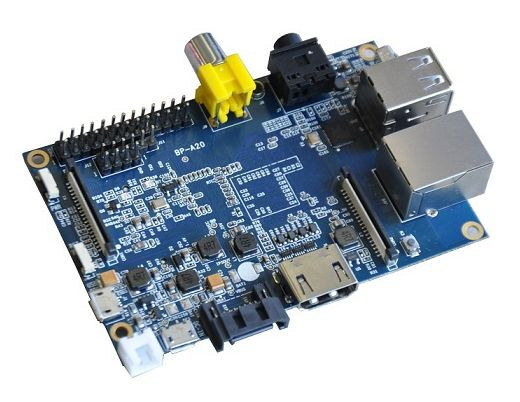
\includegraphics[width=0.5\textwidth]{content/pictures/bpim1.jpg}
\label{pic:bpim1}
\end{figure}
\begin{figure}[!htbp]
\caption{Banana Pi G1}
\source{http://www.banana-pi.com/tp/2015013018534129497.JPG}
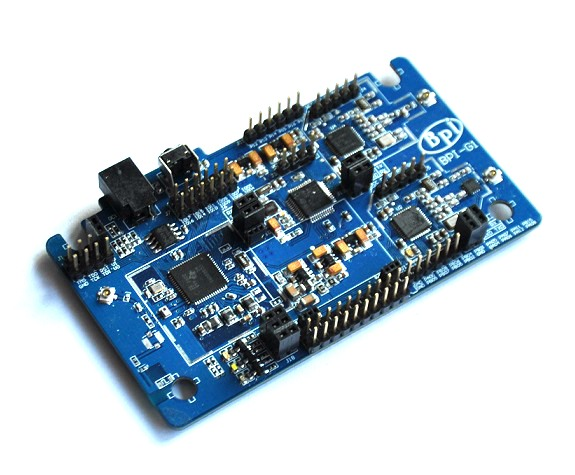
\includegraphics[width=0.5\textwidth]{content/pictures/bpig1.jpg}
\label{pic:bpig1}
\end{figure}
\begin{figure}[!htbp]
\caption{Banana Pi D1}
\source{https://upload.wikimedia.org/wikipedia/commons/c/c7/BananaPi-D1.jpg}
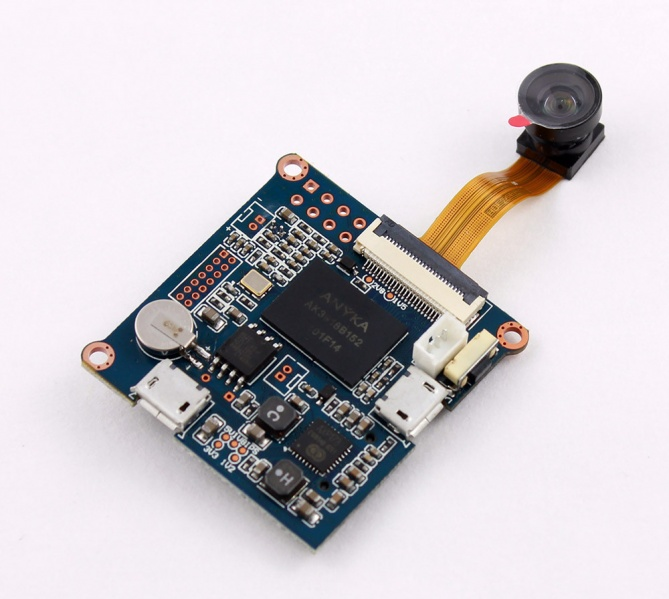
\includegraphics[width=0.5\textwidth]{content/pictures/bpid1.jpg}
\label{pic:bpid1}
\end{figure}
\begin{figure}[!htbp]
\caption{Banana Pi R1}
\source{http://www.banana-pi.com/tp/2014082202191761603.JPG}
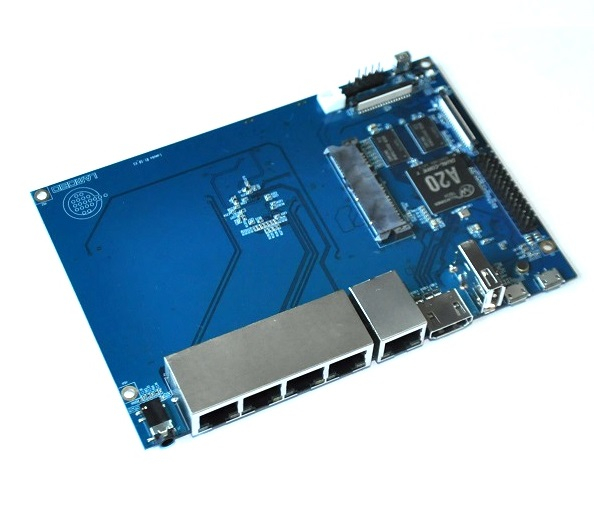
\includegraphics[width=0.5\textwidth]{content/pictures/bpir1.jpg}
\label{pic:bpir1}
\end{figure}

\section{Hersteller}


\section{Banana Pi R1}


\section{Informationsquellen}

\chapter{Auswahl und Vergleich der Betriebssysteme}


% Schalgwortverzeichnis (Index)
%\printindex

% Literaturverzeichnis
\singlespacing
\bibliographystyle{alphadin}
\bibliography{bibtex}

% Eidesstattliche Erklärung
\chapter*{Eidesstattliche Erklärung\markboth{Eidesstattliche Erklärung}{}}
% Eintrag in das Inhaltsverzeichnis 
\addcontentsline{toc}{chapter}{Eidesstattliche Erklärung}

Ich versichere, dass ich die vorstehende Arbeit selbständig verfasst und hierzu
keine anderen als die angegebenen Hilfsmittel verwendet habe. Alle Stellen der Arbeit die 
wörtlich oder sinngemäß aus fremden Quellen entnommen wurden, sind als solche kenntlich gemacht.
\\
\\
Die Arbeit wurde bisher in gleicher oder ähnlicher Form in keinem anderen
Studiengang als Prüfungsleistung vorgelegt oder an anderer Stelle
veröffentlicht.
\\
\\
Ich bin mir bewusst, dass eine falsche Erklärung rechtliche Folgen haben kann.

\vspace*{1.5cm} \par
\line(1,0){200} \par
\docOrt, \docAbgabedatum ~~\docVorname~\docNachname

%Zurücksetzen \chaptermark
\let\chaptermark\oldchaptermark

% Hier können Anhaenge angefuegt werden
\begin{appendices}
\chapter{Protokolle der Meetings}
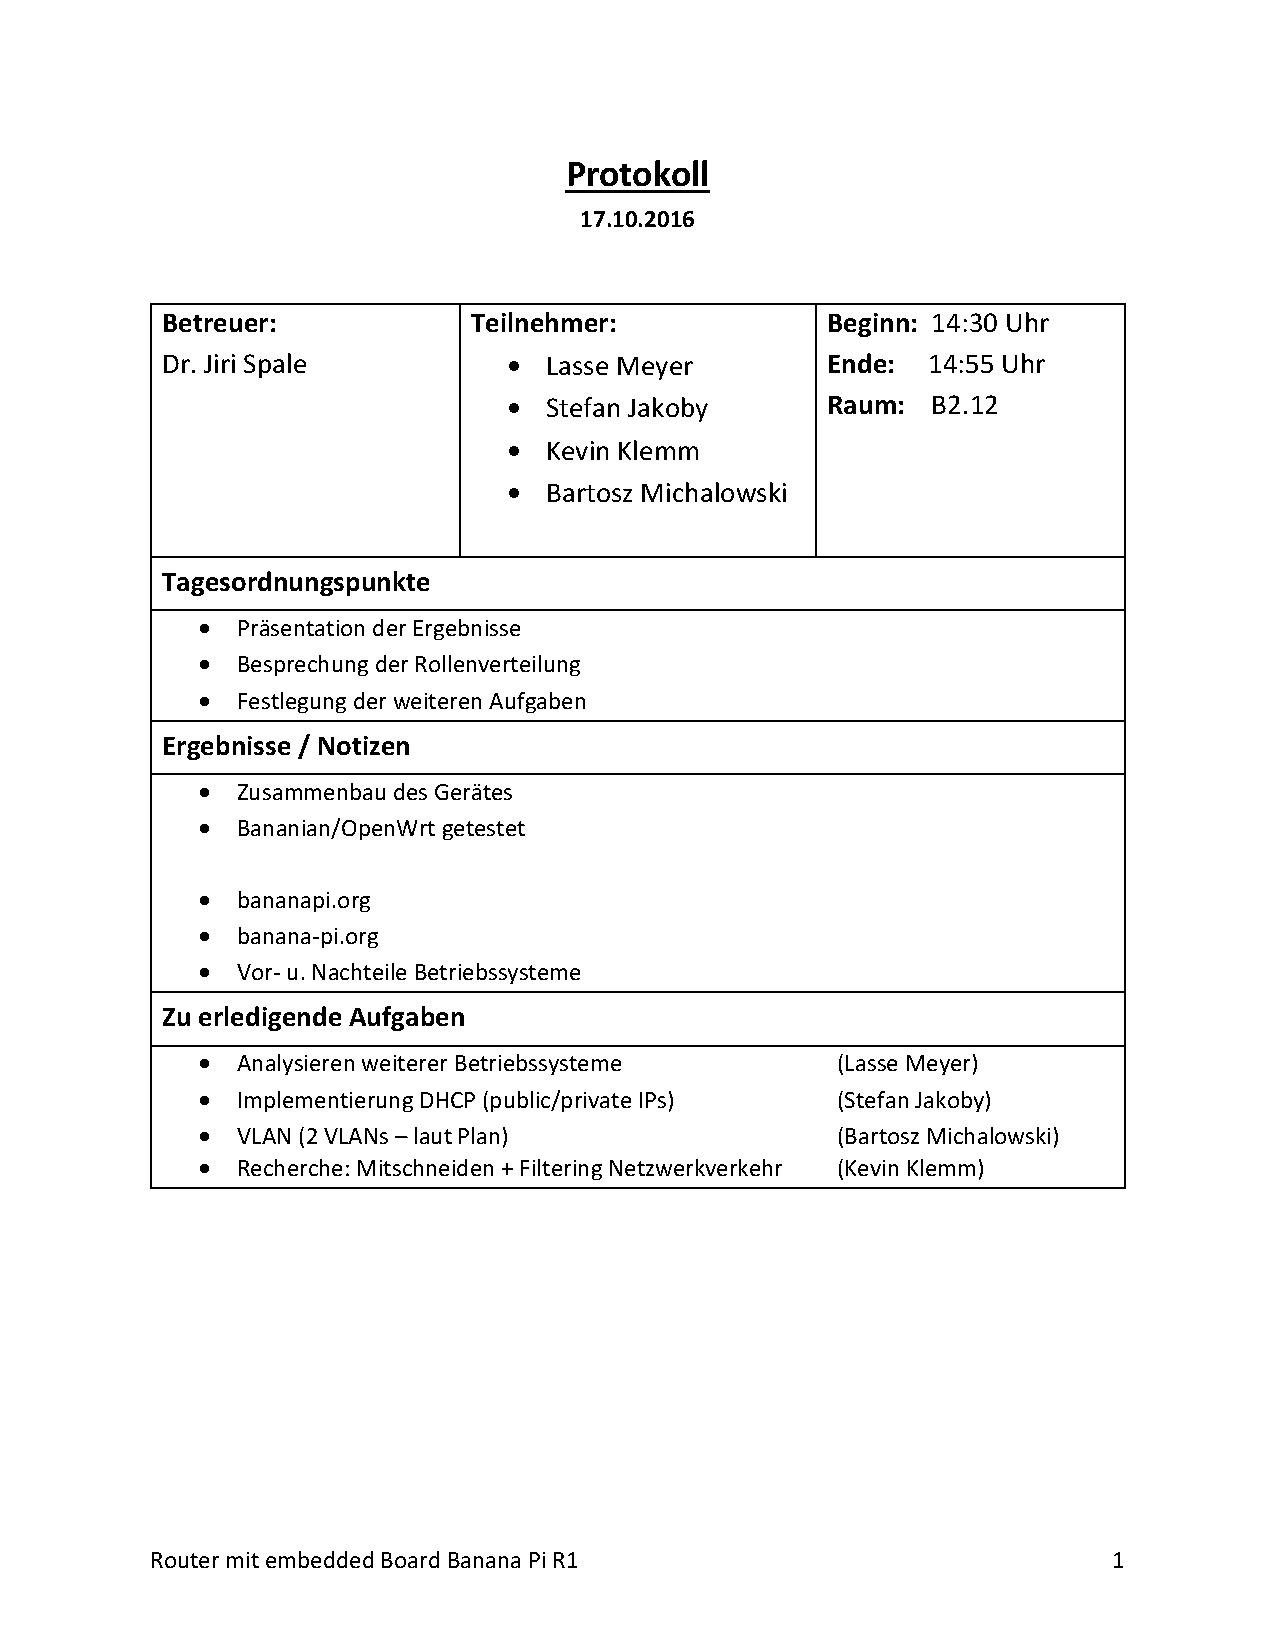
\includepdf[pages=-]{../protocols/Protokoll_17_10_2016.pdf}
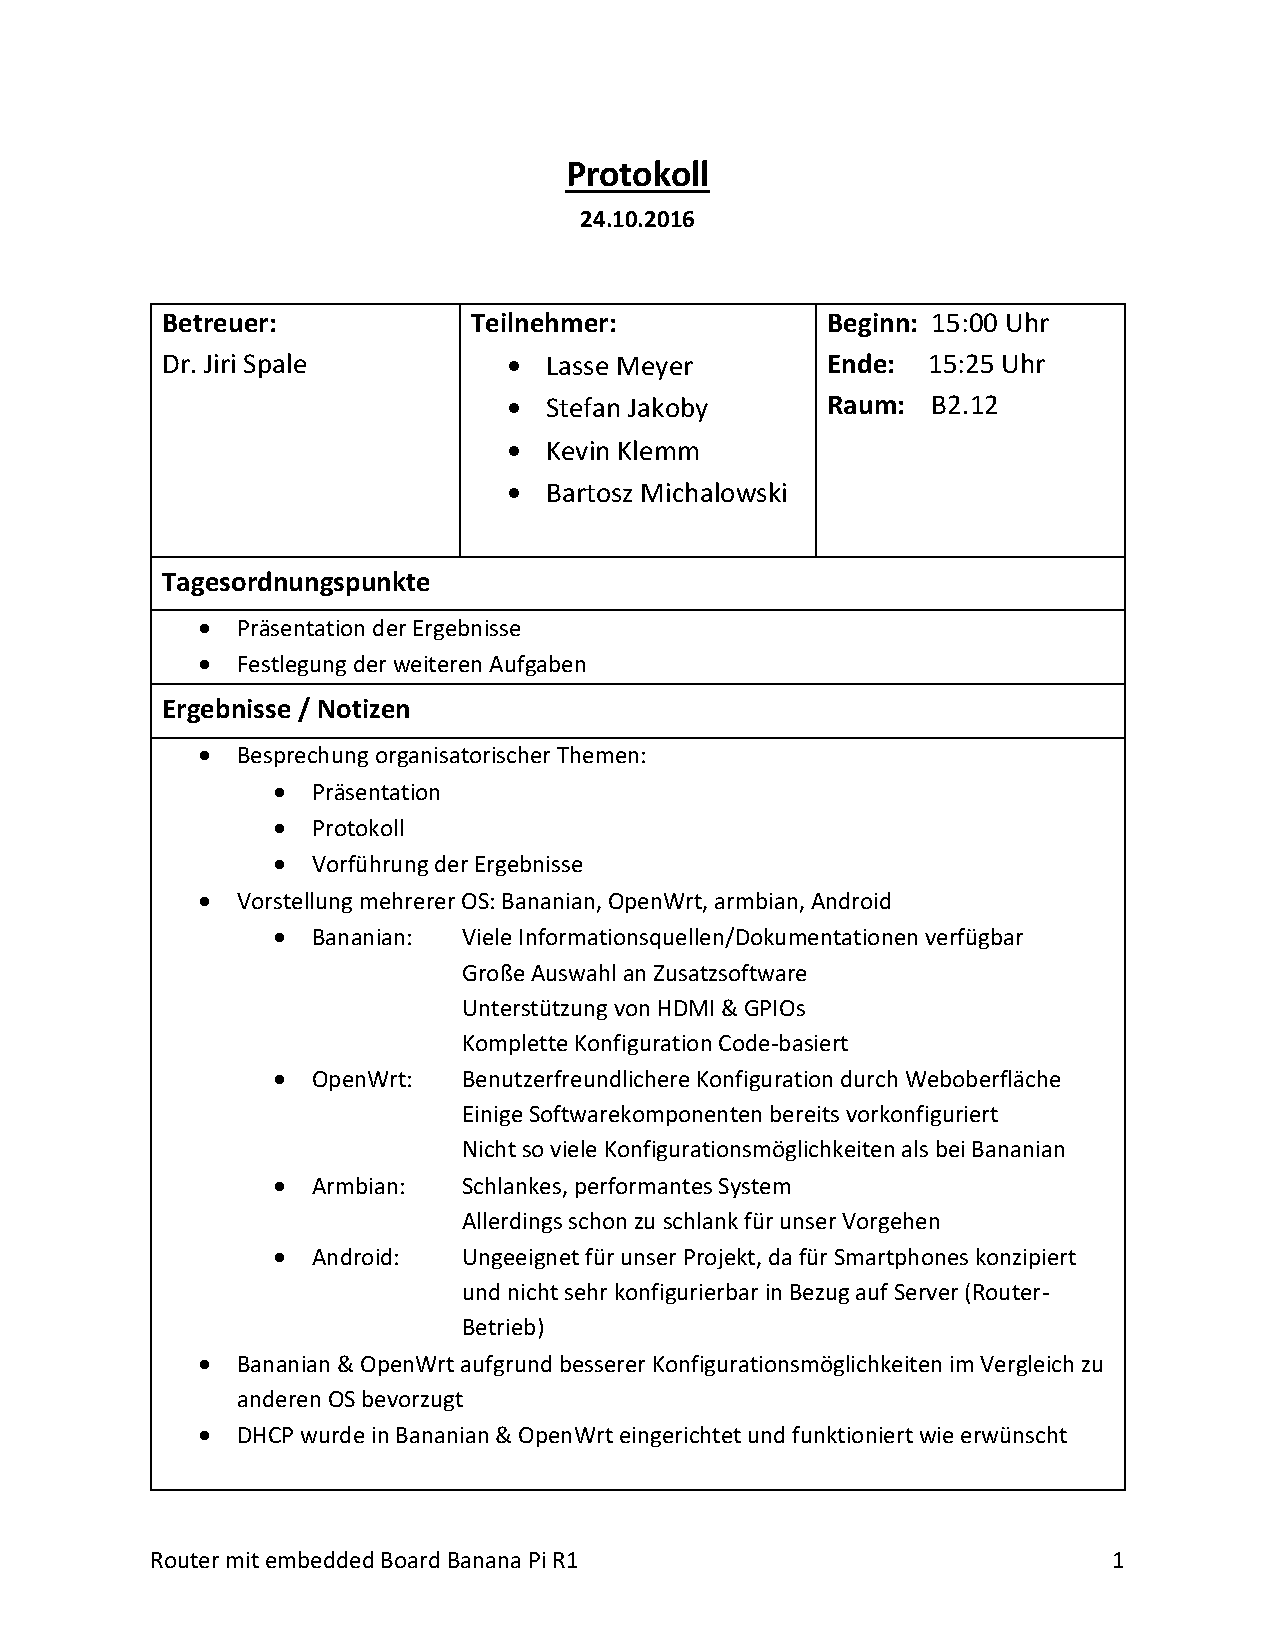
\includepdf[pages=-]{../protocols/Protokoll_24_10_2016.pdf}

\chapter{Statuspräsentationen}
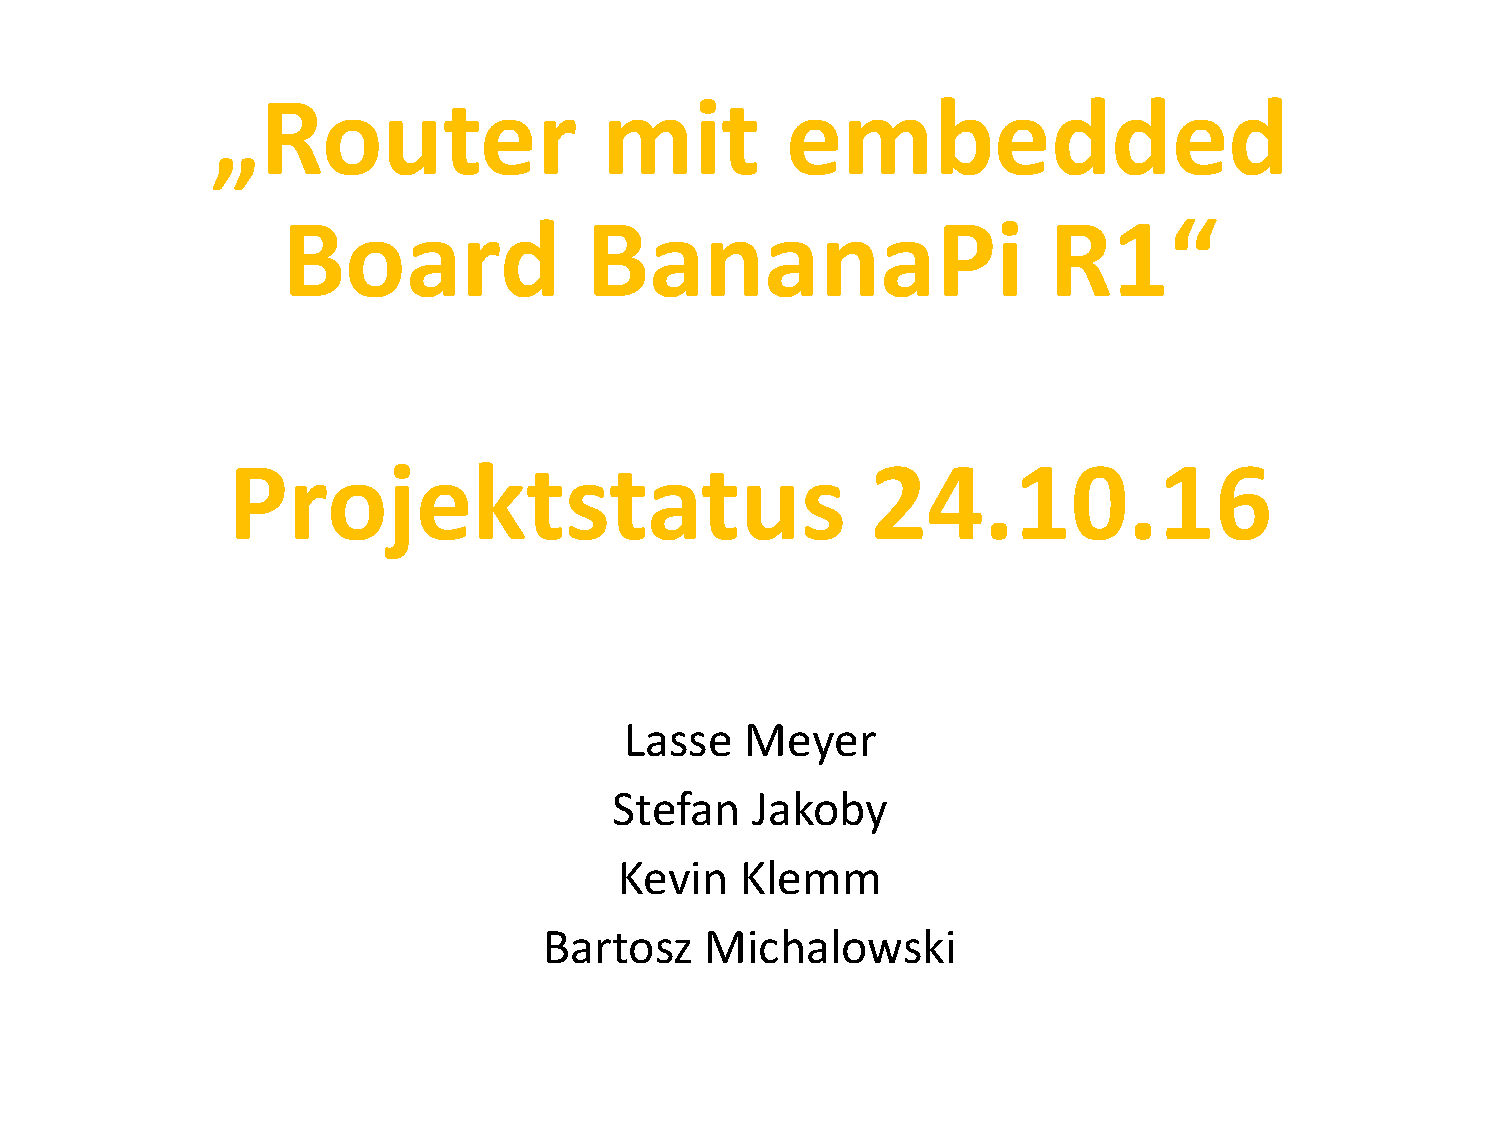
\includepdf[pages=-]{../presentations/Projektstatus_24_10_16.pdf}
\end{appendices}
\end{document}      